\chapter{Dynamics}
This is the first experiment chapter. Add your content here.

\section{Energy and Work}

The work-energy theorem states that the work done on an object equals its change in kinetic energy:

\[ W = \Delta KE = \frac{1}{2}mv_f^2 - \frac{1}{2}mv_i^2 \]

\begin{tutorialbox}[title=Creating Energy Diagrams]
Use PGFPlots for energy graphs:
\begin{verbatim}
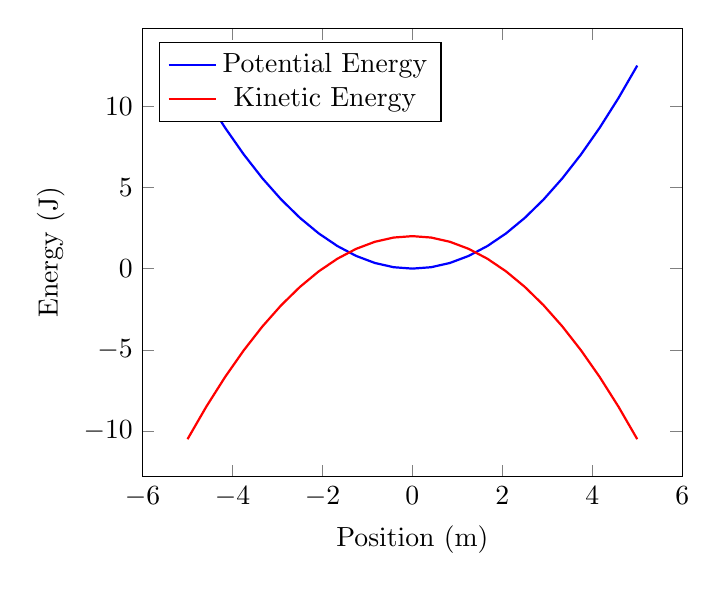
\begin{tikzpicture}
\begin{axis}[
    xlabel={Position (m)},
    ylabel={Energy (J)},
    legend pos=north west
]
\addplot[blue,thick] {x^2/2};
\addlegendentry{Potential Energy}
\addplot[red,thick] {2-x^2/2};
\addlegendentry{Kinetic Energy}
\end{axis}
\end{tikzpicture}
\end{verbatim}
\end{tutorialbox}

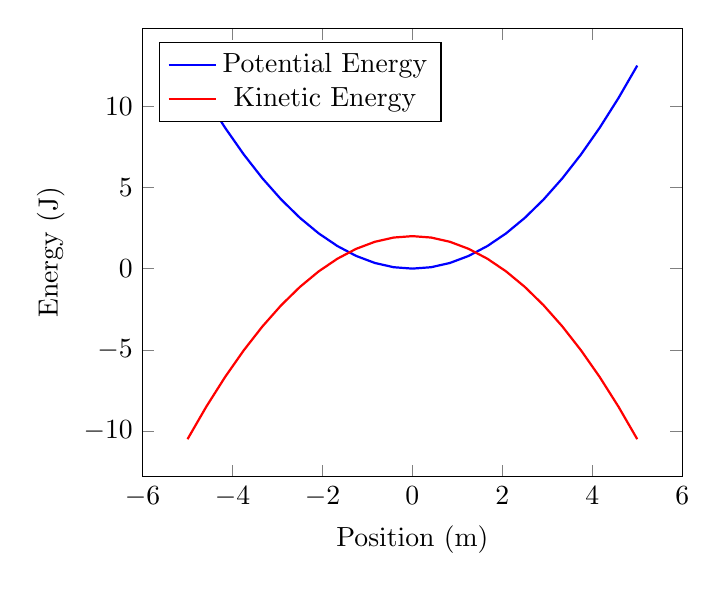
\begin{tikzpicture}
\begin{axis}[
    xlabel={Position (m)},
    ylabel={Energy (J)},
    legend pos=north west
]
\addplot[blue,thick] {x^2/2};
\addlegendentry{Potential Energy}
\addplot[red,thick] {2-x^2/2};
\addlegendentry{Kinetic Energy}
\end{axis}
\end{tikzpicture}